\documentclass[12pt,a4paper]{article}
\usepackage[utf8]{inputenc}
\usepackage[french]{babel}
\usepackage[T1]{fontenc}
\usepackage[margin=4cm]{geometry}
\usepackage{graphicx}
\usepackage{makeidx}
\usepackage{url}
\usepackage{caption}
\usepackage{subcaption}
\usepackage{enumerate}
\usepackage{enumitem}
\usepackage{ifthen}
\usepackage{amssymb}
\usepackage{dsfont}
\usepackage{multicol}
\usepackage[hidelinks]{hyperref}
\usepackage{amsmath}
\usepackage{multirow}
\usepackage{pgfplotstable}
\usepackage{booktabs}
\usepackage{csvsimple}
\usepackage[toc,page]{appendix} 

\newcommand{\figref}[1]{Figure~\ref{fig:#1}}
\newcommand{\tabref}[1]{Table~\ref{tab:#1}}
\newcommand{\secref}[1]{Section~\ref{sec:#1}}
\newcommand{\alref}[1]{Algorithm~\ref{alg:#1}}
\newcommand{\lstref}[1]{Listing~\ref{lst:#1}}
%\renewcommand{\appendixtocname}{Annexes} 
%\renewcommand{\appendixpagename}{Annexes} 


\title{\vspace{4cm}\textbf{L'impact du renommage sur les métriques de procédés}\vspace{3cm}}

\author{
Pierre Chanson\\\\
Mémoire de stage de Master2\\
Encadrants: Jean-Rémy Falleri et Matthieu Foucault\\\\
LaBRI, UMR 5800\\
F-33400, Talence, France\\\\
\texttt{Email: pierre.chanson@etu.u-bordeaux.fr,}\and
\texttt{\{falleri,mfoucault\}@labri.fr}\\
}


\begin{document}

\begin{figure}[t]
\center

\includegraphics[scale=0.25]{data/figures/UnivBordeaux.jpg}
\end{figure}
\maketitle
\newpage
\tableofcontents
\newpage
\section{Introduction}
\label{sec:intro}

L'accès aux dépôts logiciels a rendu possible de nombreux travaux de recherche sur l'évolution logicielle. Plus particulièrement, les dépôts de code source gérés par des outils de contrôle de versions (Version Control System, VCS, comme SVN, Mercurial ou encore Git) contiennent l'historique de construction d'un logiciel. Principalement dans le domaine du ``Reverse Engineering'', la compréhension des choix des développeurs lors de la création d'un logiciel, des études se basent sur l'analyse de ces historiques. Ces études entrent dans le cadre des études ``MSR'' (Minning Software Repository). De même, la prédiction de bugs, un des défis connus du Génie Logiciel dont le but est de prédire le nombre de bugs et leur localisation dans la prochaine version d'un logiciel, utilise des informations contenu dans l'historique d'un projet. Cette étude se base sur les métriques de procédés comme prédicateurs de bugs. Les métriques de procédés se concentrent sur l'évolution d'un logiciel et mesurent les modifications subies par les entités d'un code source durant leur cycle de vie. L'hypothèse principale étant que la manière dont les entités du code ont changé a un impact majeur sur la qualité de leur prédiction de bugs.\\
Or au cours de son histoire, un fichier peut être renommé et/ou déplacé dans un autre dossier du projet.\\
Théoriquement, si le renommage d'un fichier à un moment donné de son histoire n'est pas pris en compte, le calcul d'une métrique de procédé sur ce fichier sera faussé. En effet, si on identifie le fichier par son nom, on perdra les informations récoltées avant le renommage. Par ailleurs on peut penser que le refactoring, dont le renommage de fichiers, est très présent dans le développement des logiciels à succès d'aujourd'hui. En pratique, nous n'avons pas de chiffres pour le montrer.\\ 
Dans un premier temps nous effectuerons une étude de l'existant sur les méthodes utilisées pour détecter le refactoring, les logiciels qui ont été étudié, les métriques de procédés ainsi que les VCS. Puis nous choisirons un ensemble de projets cohérent pour faire nos propres expérimentations, nous définirons un niveau de granularité et nous ferons une analyse manuelle des projets choisis pour récupérer les renommages réels. Par la suite, nous définirons un modèle et nous utiliserons un outil pour récupérer les renommages. Enfin, nous définirons comment calculer certaines métriques de procédés et mesurerons l'impact du renommage. Les résultats de nos expérimentations amèneront à une publication dans la conférence ICSME 2014.\\


\section{Contexte}
\label{sec:metriques}

Nous décrivons dans cette partie comment les métriques de procédés sont calculées. Puis, nous expliquons comment les fichiers renommés peuvent avoir un impact sur ces métriques. Enfin, nous décrivons comment les VCS, actuellement, traitent le renommage.

\subsection{Calcul des métriques de procédés}

Les métriques de procédés (process metrics) mesurent les modifications subies par les entités de code source, au cours d'une période donnée dans l'histoire d'un logiciel. Une version étant un état donné de l'évolution d'un logiciel, nous définissons une période par une suite de version successive. Pour la prédiction de bugs, elles sont généralement calculées dans une période située entre deux \texttt{releases}. Une \texttt{release} correspond à la sortie d'une version dite stable du logiciel. L'objectif est de prédire les bugs qui apparaîtront lors de la prochaine version, en particulier si cette version est une \texttt{release}. Elles ne prennent alors en considération que les entités susceptibles de contenir des bugs dans la prochaine version, c'est-à-dire les entités étant toujours présentes à la fin de la période et qui ont été actives dans la période. Elles excluent entre autres les entités supprimées au cours de la période.\\

Un gestionnaire de versions (VCS) offre plusieurs moyens de calculer les métriques de procédés car il stocke les informations sur les entités modifiées à chaque nouvelle version. Les modifications apportées par une nouvelle version sont présentées sous la forme d'un \texttt{commit}. Voici un exemple de \texttt{commit} lambda.\\

\begingroup
	\fontsize{8pt}{12pt}\selectfont
	\centering\begin{boxedverbatim}
	commit 3d87c26845095438b6c946dc4e1029280593fb91	
	Author: Aaron Patterson <aaron.patterson@gmail.com>
	Date:   Fri May 2 11:52:37 2014 -0700

	    push up bind params on "simple" subquery calculations 
	    bind parameters we not being propogated to simple subquery 
	    calculation calls. This fixes it

	 activerecord/lib/active_record/relation/calculations.rb            |    6 ++++--
	 activerecord/test/cases/associations/has_many_associations_test.rb |    8 +++++++-
	 2 files changed, 11 insertions(+), 3 deletions(-)
	\end{boxedverbatim}
\endgroup
\linebreak

On peut y retrouver les informations suivantes: 
\begin{itemize}
\item L'identité du \texttt{commit} (une \texttt{SHA-1} ici).
\item L'auteur de ces modifications.
\item La date du \texttt{commit}.
\item Le commentaire.
\item Des détails sur les entités (ici des fichiers) qui ont été modifiées.\\
\end{itemize}

Un VCS permet aussi la récupération du contenu de chaque entité et de l'ensemble d'un projet à partir d'une version donnée qu'on appelle un \texttt{``snapshot''}. Pour calculer ces métriques, il est donc possible d'analyser chaque entité modifiée lors d'une période puis de garder uniquement les entités toujours présentes à la dernière version de notre période.\\

Plus précisément, voici comment un VCS peut être utilisé pour calculer une métrique de procédé: 
\begin{enumerate}
\item Nous récupérons d'abord la dernière version du projet pour obtenir les entités existantes à la fin de la période considérée. On note $A$ cet ensemble d'entités.
\item Nous récupérons toutes les modifications effectuées durant la période. On note $C$ l'ensemble des modifications dans l'ordre chronologique.
\item Troisièmement, nous parcourons cet ensemble de modifications en commençant par la plus ancienne ($c_0 \in C$) jusqu'à la plus récente ($c_n \in C$) dans le but de calculer la métrique de procédé pour chaque entité.
\end{enumerate}

Dans ce rapport, nous considérons les trois métriques de procédés les plus utilisés données par Radjenovic \emph{et al}~\cite{radjenovic_software_2013}. le nombre de développeurs (NoD), le nombre de modifications (NoC) et le Code Churn (CC). Nous expliquons alors comment calculer ces métriques:
On note $\mu_{a}^{M}$ la valeur de la métrique $M$ pour l'entité $a$ et  $c_i$ la modification courante lors du parcours. 
\begin{description}
	\item[NoD] (nombre de développeurs) Pour chaque entité $a$ pointé par $c_i$ qui appartient aussi à $A$ ($a \in A$), on ajoute à $\mu_{a}^{NoD}$ le nombre d'auteurs qui ont effectué les modifications $c_i$ et qui ont modifié $a$ pour la première fois dans la période.
	\item[NoC] (nombre de modifications) Pour chaque entité $a$ pointé par $c_i$ qui appartient aussi à $A$ ($a \in A$), on ajoute $1$ à $\mu_{a}^{C}$ tel que $c_i$ indique qu'une nouvelle modification a été effectuée.
	\item[CC] (Code Churn) Pour chaque entité $a$ pointé par $c_i$ qui appartient aussi à $A$ ($a \in A$), on vérifie d'abord que la modification n'est pas une création d'entité. Si c'est le cas, cela signifie que l'entité a été créée durant la période, donc on initialise son $\mu_{a}^{CC}$ à son nombre de lignes. Ensuite au prochain $c_j$ qui cible $a$ dans la période avec ($i < j$), on compare les deux versions et on ajoute à $\mu_{a}^{CC}$ le nombre de lignes ajoutées ou supprimées.
\end{description}


\subsection{Métriques de procédés et renommage}

Un VCS est donc particulièrement utile dans cet exercice. Cependant, il faut noter que la plus part des VCS identifient une entité par son chemin $+$ son nom. Le chemin représente l'ensemble des dossiers parents depuis la racine du projet. On en déduit qu'un renommage du fichier ou d'un dossier, aura un impact sur le calcul des métriques. Pour expliquer cet impact, il est présenté un exemple d'historique d'un logiciel. (\figref{example}) . Ce projet ne contient qu'une entité, Test.php, qui est renommé en Hello.php dans la dernière version. Dans cet exemple, nous calculons les trois métriques NoD, NoC et CC entre les versions 1 et 3.\\

\begin{figure}[t]
	\centering
	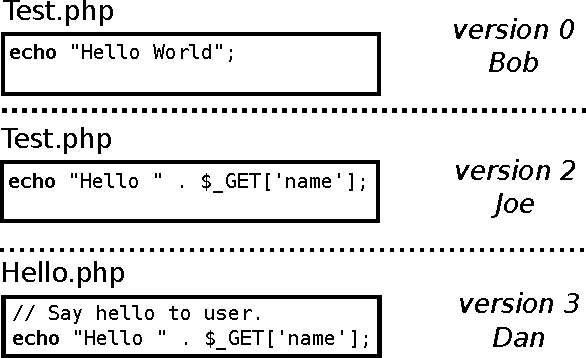
\includegraphics[width=0.8\linewidth,keepaspectratio]{data/figures/example.pdf}
	\caption{Exemple d'un historique de projet. Le projet est composé d'un seul fichier \texttt{Test.php} qui est renommé en \texttt{Hello.php} dans la dernière version.}
	\label{fig:example}
\end{figure}

La dernière version de la période ne contient qu'une entité, \texttt{Hello.php}. C'est donc cette entité qui sera considérée uniquement, par les approches qui visent à prédire les bugs. Si on ne prend pas en compte le renommage, l'entité n'apparaît que dans la version 3. Ainsi, le calcul est trivial, étant donné qu'il n'y a qu'un seul développeur, alors $\mu^{NoD}=1$. Il n'y a qu'une seule modification, la creation du fichier \texttt{Hello.php}, donc $\mu^{NoC}=1$. La création du fichier implique l'ajout de deux lignes de codes donc $\mu^{CC}=2$.\\

Par ailleurs, en prenant en compte le fait que ce fichier a été renommé, il y a trois versions à considérer qui ciblent notre entité. Le premier nom du fichier était \texttt{Test.php}. Les valeurs des métriques de procédés changent donc complètement. Ce fichier a eu un premier auteur lors de la version $1$ puis un deuxième à la version $2$. Le fichier est ensuite renommé en Hello.php par un troisième auteur donc $\mu^{NoD}=3$. Le fichier a subi trois modifications: la création du fichier version $1$, une modification du contenu version $2$ et un renommage version $3$ donc $\mu^{NoC}=3$. Enfin, pour le Code Churn, la création du fichier implique l'ajout d'$1$ ligne de code, la modification de cette ligne version $2$ implique la suppression d'$1$ ligne plus l'ajout d'$1$ ligne de code et la version 3, l'ajout d'$1$ ligne de commentaire. Nous avons donc maintenant $\mu^{CC}=4$. \\

Notre exemple montre que le renommage d'entité de code source peut biaiser le calcul des métriques de procédés. Plus généralement, lorsque le renommage est pris en compte, les valeurs des métriques NoD et NoC ne peuvent qu'avoir une valeur plus grande. En effet, plus une entité est ancienne plus elle a de chances d'avoir un nombre de développeurs et un nombre de modifications élevés. La valeur du Code Churn quant à elle, peut augmenter ou diminuer si le renommage est pris en compte. En effet, comme nous l'avons vu dans l'exemple précédent, un renommage d'entité est considéré comme la suppression d'une entité et l'ajout d'une nouvelle entité si le renommage n'est pas pris en compte. Le renommage d'une entité dans une période induit donc que l'entité renommée a été créée durant la période. Cela entraine l'ajout du nombre de lignes de la nouvelle entité à la métrique CC, à la version où elle a été renommée. Ainsi, si l'entité est considérable, son CC sera bien plus important qu'il ne devrait. 

Un autre effet intéressant à remarquer est que plus une entité est renommée proche de la fin de la période, pire sera l'effet. En particulier, si elle est renommée juste avant la dernière version, alors tous les changements préalables qu'elle a subis seront perdus.\\

\subsection{Renommage et VCS}
  
Nous avons effectué une analyse approfondie des principaux VCS (CVS, Subversion, Git and Mercurial) dans le but de décrire les mécanismes qu'ils proposent pour traiter le renommage. 

Tous ces VCS sont à une granularité d'entité au niveau fichier. Comme expliqué précédemment, les entités sont identifiés par leur chemin absolu, c'est-à-dire le chemin depuis la racine du projet $+$ leur nom. Pour tous ces VCS, une modification dans le chemin d'un fichier, qui peut être due à un changement d'emplacement dans les dossiers ou à un changement de son nom, est considérée comme une suppression de fichier et création de fichier. Certains VCS proposent en complément un mécanisme pour traiter les renommages. Ce mécanisme peut être manuel ou automatique. Un mécanisme de traitement de renommage est dit manuel lorsque le développeur doit utiliser une commande particulière pour indiquer que la modification effectuée sur le fichier est un renommage. Un mécanisme est automatique lorsque le VCS propose un algorithme qui peut automatiquement détecter le renommage. De plus, ce mécanisme automatique peut être appliqué par défaut par le VCS ou de manière optionnelle lorsque le développeur doit explicitement ajouter une option de commande dans sa recherche dans l'historique.\\
 
La ~\tabref{vcs} résume notre étude. Alors que CVS ne gère pas du tout le renommage, SVN ou Mercural propose un mécanisme manuel de détection de renommage de fichiers. Git quant à lui propose un algorithme de détection de renommage automatique mais optionnel. Aucun de ces VCS ne propose un mécanisme automatique par défaut.\\ 

%Cependant, nous allons voir que le traitement du renommage de ces VCS ne parvient pas à limiter l'impact sur le calcul des métriques de procédés.\\ 

\begin{table}[h]
\centering
\begin{tabular}{rccc}
\toprule
 & \multicolumn{3}{c}{Traitement du renommage}\\
\cmidrule{2-4}
& & \multicolumn{2}{c}{Automatique}\\
\cmidrule{3-4}
Outil & Manuel & Standard & Optionnel\\
\midrule
CVS & & &\\
Subversion & $\times$ & &\\
Mercurial & $\times$ & &\\
Git & & & $\times$\\
\bottomrule
\end{tabular}
\caption{Traitement du renommage des principaux VCS.}
\label{tab:vcs}
\end{table}

Pour les VCS qui utilisent une détection manuelle, cela implique que c'est aux développeurs d'utiliser les commandes appropriées. Cependant, certaines études montrent que les développeurs n'utilisent pas ces commandes systématiquement. Le renommage peut être effectué jusqu'à $89\%$ du temps sans utiliser les commandes adaptées ~\cite{lavoie_inferring_2012,steidl_incremental_2014}. De plus, l'étude de Kim et al ~\cite{kim_field_2012} montre que $51$\% des développeurs n'utilisent pas les commandes prévues par le VCS pour le \textit{refactoring} (incluant le renommage). Ces trois études effectuées sur des projets open-source et industriels, montrent qu'il est risqué de compter sur le fait que les développeurs utilisent les commandes adéquates pour le refactoring.\\

Git étant le seul VCS à proposer un traitement automatique optionnel du renommage, il est donc le seul sur lequel nous pouvons compter pour nos expérimentations futures. Nous le considérerons dorénavant comme notre VCS de référence. 

Par ailleurs, le traitement automatique optionnel du renommage nécessite une certaine connaissance des paramètres internes du VCS, notamment afin de choisir la bonne option pour gérer le renommage. Cependant, nous n'avons jamais trouvé d'explications à propos de la configuration d'un VCS et de ses options, dans aucune étude ayant pour but la prédiction de bug avec l'utilisation de métriques de procédés. En effet, comme nous le décrivons dans la Section 5, dans notre analyse des études passées, aucune d'elle n'a jamais utilisée Git comme gestionnaire de version, le seul à proposer un traitement automatique optionnel du renommage.\\

Le mécanisme proposé par Git utilise un algorithme nommé ``Origin Analysis''.

\subsection{``Origin Analysis''}

Nous expliquons ici succinctement l'algorithme utilisé par Git pour la détection de renommage de fichiers. Celui-ci est connu sous le nom de ``Origin Analysis'' et est expliqué par Godfrey \emph{et al} ~\cite{tu_integrated_2002,godfrey_tracking_2002,godfrey_using_2005}.\\

Tout d'abord, il faut considérer deux versions successives d'un projet. Une version est composée d'un ensemble d'entité (fichiers, fonctions..). D'une version à la suivante, certaines entités peuvent être modifiées, certaines supprimées et d'autres ajoutées. 

\begin{figure}[h]
  \centering
  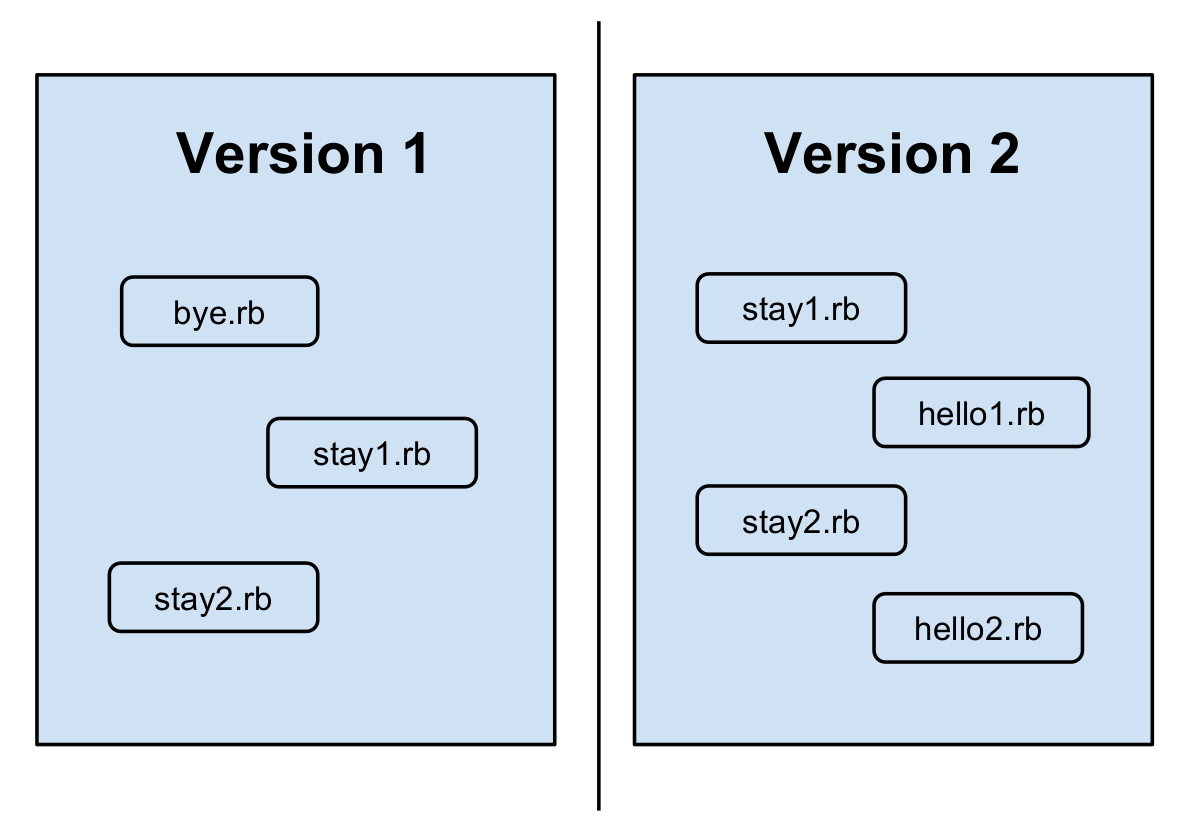
\includegraphics[scale=0.5]{data/figures/oa.png}
	\caption{Schématisation de deux versions consécutives.}
	\label{fig:oa}
\end{figure}

L'analyse proposée par Godrey pour détecter les renommages d'une version à la suivante est basée sur le principe d'une analyse de ``Bertillonnage''~\cite{bertillonnage}. Cette analyse a pour but de trouver l’origine possible d’une entité apparemment ``nouvelle''. Elle consiste à comparer entre elles les entités composantes de chaque paire possible ``entité supprimée, entité créée'', de version consécutive.\\ 

Le schéma donné en~\figref{oa} représente le contenu d'un projet à deux versions consécutives. Si on observe la différence entre la version 1 et la version 2, on remarque que le fichier \texttt{src/bye.rb} a été supprimé alors que les fichiers \texttt{src/hello1.rb} et \texttt{src/hello2.rb} ont été ajoutés.
Dans cet exemple, l'analyse de Godfrey mettrait en corrélation les paires \texttt{(src/bye.rb, src/hello1.rb)} et \texttt{(src/bye.rb, src/hello2.rb)}.\\  

Cette comparaison s'effectue grâce à un choix et un nombre de métriques défini par l'utilisateur (en l'occurrence Git). Pour chaque paire d'entités, la distance Euclidienne est calculée. Elle nous donne la distance dans l’espace $nD$ (pour les $n$ métriques). Combinée avec une technique de comparaison des noms des entités, nous obtenons une liste ordonnée des renommages potentiels. Un seuil d'acceptabilité peut alors être défini pour juger si un couple compose un renommage d'entité.

Git met en application cette analyse avec un seuil d'acceptabilité établi par défaut mais qui peut être configuré à postériori.\\

% Par la suite, les analyses de Godfrey sont des améliorations de la première analyse, mais qui ne sont efficaces qu'à un niveau de granularité plus bas, c'est à dire une finesse d'analyse plus précise, en l'occurence au niveau des fonctions. Par exemple, l'analyse des dépendances qui traque les appels de fonctions, en comparant les fonctions appelantes et appelées. Ces analyses sont basées sur plusieurs types de seuils d'acceptabilité devant à chaque fois être défini par l'utilisateur. Plus Godrey améliorera ces analyses, en prenant en compte par la suite les splits et merges de fonctions (algorithme inefficace au niveau des fichiers), plus l'utilisateur sera sollicité.\\



\section{Méthodologie}
\label{sec:methodologie}

Nous présentons ici le déroulement de nos expérimentations qui consistent à étudier le phénomène du renommage et son impact sur le calcul des métriques de procédés. L’objectif étant d’évaluer si le renommage peut biaiser de manière significative les valeurs des métriques de procédés.\\

Le but de la première expérience et de calculer la quantité de renommage durant les périodes de développement. S’appuyant sur cette première expérience, notre deuxième expérience fournit une analyse de l’impact du renommage sur les métriques de procédés dans le pire des cas. \\

\subsection{Corpus}

Nous avons sélectionné un ensemble de projets sur lesquels effectuer nos expérimentations qui respectent le modèle défini. Des projets open-source, conséquents et connues de la communauté MSR. Nous avons un ensemble de projets utilisés par l'équipe de Génie Logiciel au LaBRI qui respectent le modèle avec des branches de maintenances identifiées. Les $5$ projets qui sont donnés \tabref{projects} forment un corpus pour notre prochaine expérience. Il comprend différents langages de programmation ainsi qu'un nombre de lignes de code et un nombre de développeurs moyennement élevés à évélevés par rapport aux projets open source utilisés couramment par la communauté. Les $5$ projets sont gérés sur Git afin de profiter de la détection automatique des renommages (section). 

De plus, il faut noter que nous avons choisi d'exclure tous les fichiers qui ne sont pas du code source du corpus étant donné que les métriques de procédés sont habituellement uniquement calculées sur ces fichiers. \\

\begin{table*}[h]
\centering
\small
\begin{tabular}{rllp{1.7cm}c}
\toprule
Project & Main language & Size (LoC) & Number of developers & URL\\
\midrule
Jenkins & Java & 200851 & 454 & \url{github.com/jenkinsci/jenkins} \\
JQuery & JavaScript & 41656 & 223 & \url{github.com/jquery/jquery} \\
PHPUnit & PHP & 21799 & 152 & \url{github.com/sebastianbergmann/phpunit}\\
Pyramid & Python & 38726 & 205 & \url{github.com/Pylons/pyramid} \\
Rails & Ruby & 181002 & 2767 & \url{github.com/rails/rails}\\
\bottomrule
\end{tabular}
\caption{Notre corpus de projets.}
\label{tab:projects}
\end{table*}

\subsection{Première expérience}

Nous définissons maintenant le modèle \figref{model}, que les projets que nous allons analyser devrons respecter. Ce modèle représente une architecture pour le dépôt de code source dérivé de l'architecture Git Flow.\\

\begin{figure}[h]
  \centering
  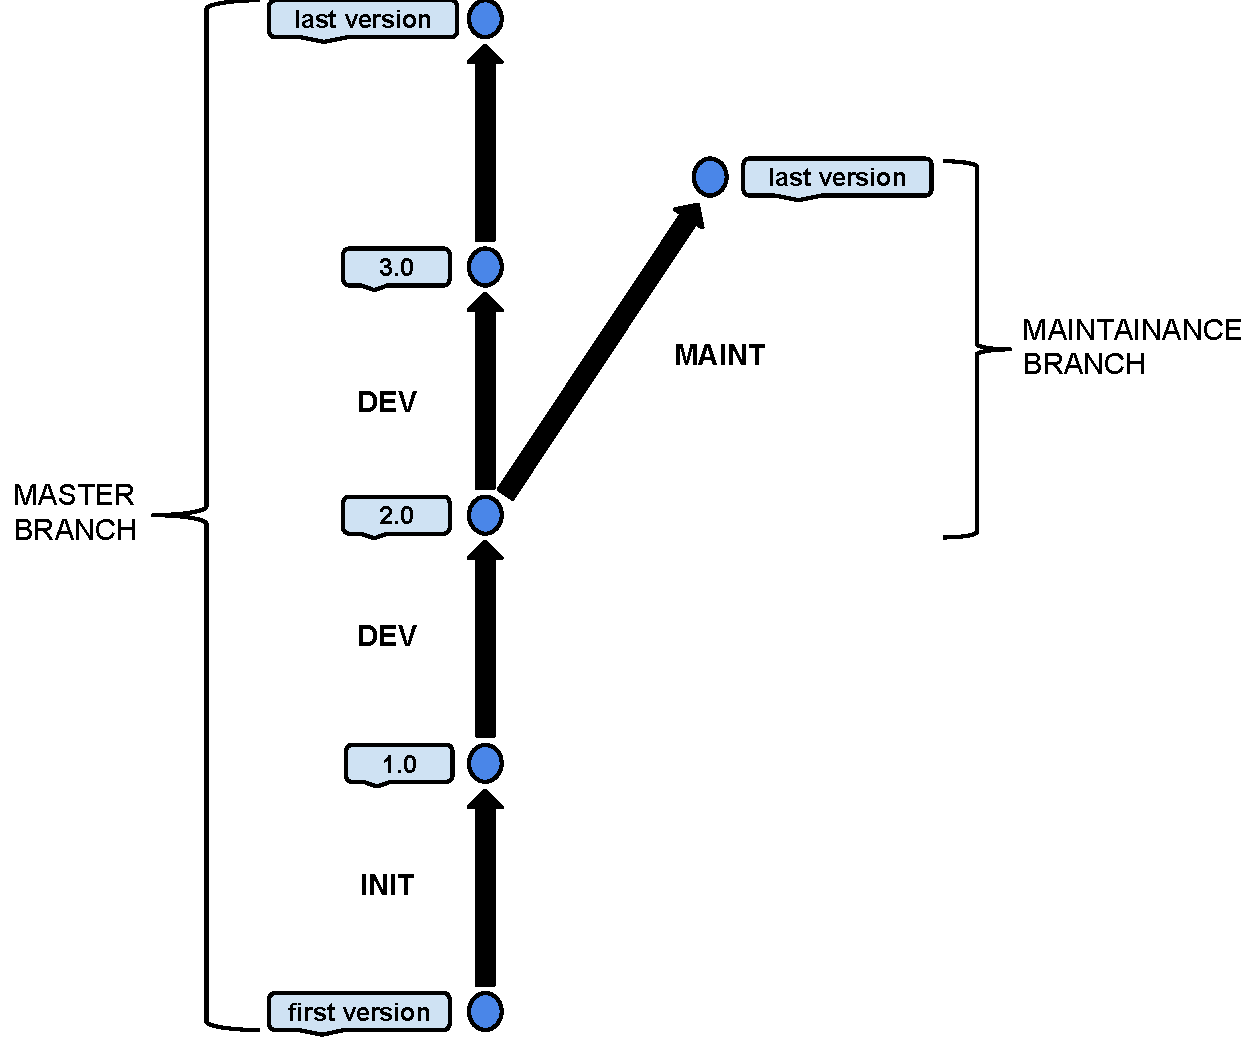
\includegraphics[scale=0.5]{data/figures/periods.pdf}
	\caption{Modèle d'architecture de dépot de code source}
	\label{fig:model}
\end{figure}

Les projets de développement logiciel suivent généralement des phases distinctes durant leur cycle de vie. Habituellement une période de développement commence avant qu'une première release soit accessible aux utilisateurs, puis cette release est maintenue pendant qu'une autre se prépare et ainsi de suite.

Nous avons ainsi deux types de branches, les branches de maintenance et la branche master. Nous divisons les branches en périodes, c'est-à-dire en une séquence de commits, la branche master contient une période initiale (init) entre la première version du logiciel (incluse) et la première release, puis des périodes de développement (dev) entre chaque release. Chaque projet contient des releases majeures, qui correspondent à des points-clés du projet, des périodes susceptibles de contenir beaucoup de changements, et des releases mineures. On distingue les releases majeures des mineures par une augmentation significative du numéro de release. Par exemple $1.9-2.0$ pour Jquery, $3.7-4.0$ pour PHPUnit ou $0.13-1.0$ pour Rails. De l'autre côté les branches de maintenance sont divisées en périodes (maint) entre chaque release.\\

 L'objectif de notre première expérience est de mieux comprendre le renommage d'entités. En particulier, d'observer quand les renommages apparaissent et en quelle quantité. Nous avons donc analysé chaque période comme décrites précédemment sur chaque projet de notre corpus. Nous comptons donc sur la détection automatique de renommage de Git et l'utilisons dans notre outil développé en Ruby pour obtenir nos chiffres (détails dans la section résultats). (TODO pourquoi Ruby ?) Nous suivons ces trois étapes entre chaque période:
\begin{enumerate}
\item On liste les fichiers existant à la fin de la période.
\item Pour chacun de ces fichiers, on extrait sa séquence de modification durant la période en activant la détection de renommage (commande \texttt{git log -M})
\item On calcule à partir des informations receuillies. Par exemple le pourcentage de fichiers $\%F_{R}$ qui ont été renommés au moins une fois durant la période.
\end{enumerate}
\medskip

À notre connaissance, il n'existe pas d'évaluation empirique de l'algorithme utilisé par Git pour détecter les renommages. Néanmoins, nous procédons à une évaluation manuelle de son comportement dans la partie conclusion et nous n'avons pas noté de faux positif sur 100 renommages aléatoire récupérés par notre outil.\\

\subsection{Deuxième expérience}

L'objectif de la deuxième expérience est de voir si le renommage peut biaiser significativement les valeurs des métriques de procédés décrites ci-dessus. Pour ça, nous effectuons une analyse dans le pire des cas.(TODO expliquer ?) On sélectionne la période de nos projets qui a la plus grande valeur de fichiers renommés en excluant la période initiale qui n'est généralement pas observée dans les études. Nous calculons ensuite les trois métriques avec et sans le renommage de fichiers pris en compte, puis nous calculons la corrélation de coefficient de Spearman entre les métriques avec et sans la détection de renommage. Un coefficient élevé, proche de $1$, indiquera que les métriques avec et sans détection de renommage sont très similaires alors qu'un coefficient plus petit, 0.5 et moins, indiquera que les métriques avec et sans détection de renommage sont très différentes.\\  

\section{Resultats}
\label{sec:resultats}

\subsection{resultats première expérience}

\subsection{resultats deuxième expérience}

\section{Analyse des études antérieures}
\label{sec:analyse}

Dans cette partie, nous procédons à l’analyse d’études antérieures sur la prédiction de bugs qui ont utilisé les métriques de procédés pour la prédiction de bugs. Nous évaluons si les valeurs des métriques de procédés pourraient être biaisées en regardant la façon dont ils ont recueilli leurs données.\\
Enfin, nous donnons quelques lignes de conduite à suivre pour aider les chercheurs et développeurs à éviter l’impact que le renommage d’entités pourrait avoir sur les métriques de procédés.  

\subsection{Analyse des études antérieures}

Premièrement, comme nous l'avons montré dans la \secref{results}, il est important de remarquer que les périodes contenant un taux de fichiers renommés élevés sont rares. Ainsi, la majeure partie des études antérieures ne devraient pas être affectées par ce phénomène. De plus, même dans le cas d'analyses sur des périodes contenant un taux élevé de fichiers renommés, les résultats de ces analyses pourraient également être améliorés, car les métriques de procédés auraient probablement été sous-estimées. Toutefois, plusieurs études antérieures peuvent être affectées par le renommage, comme nous le signalerons dans la suite de cette section. Quantifier de tels effets sur les études antérieures est hors de portée de notre sujet, mais nous fournissons tout de même certaines lignes de conduite à respecter pour les études futures dans \secref{guidelines}.\\

Dans notre examen des études antérieures, nous n'analysons que $26$ des articles référencés dans ~\cite{radjenovic_software_2013}. Les articles qui utilisent les trois métriques de procédés, CC, NoD ou NoC. Cependant, certaines des autres études référencées dans cet article utilisent d'autres métriques de procédés et pourraientt donc aussi être affectées par le renommage.\\

$15$ de ces études analysent des projets industriels, ~\cite{arisholm_systematic_2010,graves_predicting_2000,khoshgoftaar_using_2000,layman_iterative_2008,munson_code_1998,nagappan_use_2005,nagappan_influence_2008,nagappan_using_2007,nagappan_using_2006,nagappan_change_2010,nikora_building_2006,ostrand_programmer-based_2010,weyuker_too_2008,weyuker_using_2007,yuan_application_2000}. Aucune de ces études ne parle de renommage. Mais le manque d'informations récoltées sur les VCS utilisés et sur le projet en lui-même, ne nous permet pas de savoir si le renommage pouvait avoir un impact sur ces projets. Néanmoins, l'article de Kim et al ~\cite{kim_field_2012} explique que les développeurs dans son étude effectuent des opérations de refactoring, dont du renommage, sans utiliser les outils du VCS appropriés. Ainsi, ces études pourraient être impactées par le renommage en fonction des outils utilisés et des habitudes de développement.\\

$11$ études analysent des logiciels open-source \cite{dambros_relationship_2009,bacchelli_are_2010,caglayan_merits_2009,dambros_evaluating_2012,dambros_evaluating_2012,dambros_extensive_2010,illes-seifert_exploring_2010,li_finding_2005,matsumoto_analysis_2010,moser_analysis_2008,moser_comparative_2008,schroter_if_2006}. Les VCS utilisés dans ces études sont CVS ou Subversion. CVS ne gère pas le renommage et Subversion uniquement de manière manuelle ce qui est dangereux comme expliqué dans l'article ~\cite{lavoie_inferring_2012,steidl_incremental_2014}. Seulement deux de ces études ~\cite{moser_analysis_2008,moser_comparative_2008} parlent de renommage, dans leur set de données ou dans les ''Threats to validiy''. Pour réduire le risque d'erreur dans leurs expérimentations, ces deux études ont supprimé systématiquement tous les fichiers ajoutés ou supprimés durant les périodes analysées. C'est un bon moyen d'éviter de calculer des métriques de procédés biaisés, mais cela implique aussi de supprimer inutilement du jeu de données un nombre significatif de fichiers.\\

\subsection{Lignes de conduite}
\label{sec:guidelines}

Les résultats de nos deux expérimentations nous permettent de déduire de simples lignes de conduite pour calculer les métriques de procédés. Voici donc nos recommandations: 
\begin{itemize}
\item Eéviter de calculer ces métriques durant les périodes intitiales. En effet, ces périodes contiennent habituellement une quantité de renommage significative. Comme nous l'avons vu, les deux périodes majeures et mineures peuvent contenir un beaucoup de renommage, bien que les releases majeures semblent plus sujettes au renommage. 
\item Utiliser systématiquement un algorithme de détection de renommage, afin d'éviter d'analyser les mauvaises périodes. Git propose un algorithme dédié qui semble avoir une bonne précision, mais un rappel inconnu. Par conséquent, l'utilisation de projets gérés avec Git parrait la méthode la plus simple pour diminuer les risques du renommage. Des algorithmes de détection plus avancés sont décrits dans la littérature ~\cite{antoniol_automatic_2004,lavoie_inferring_2012,steidl_incremental_2014}. Ils ont étés validés par des études empiriques donc ils pourraient réaliser une analyse meilleure que celle de Git. 
\item Pour les métriques de procédés calculées à des niveaux de granularité plus fin que celui des fichiers, utiliser les algorithmes d``Origin Analysis'' tels que ~\cite{wu_aura:_2010}. Ces algorithmes sont efficaces au niveau de granularité des fonctions.
\item Le renommage d'entités peut être un risque important, penser à indiquer systématiquement comment il a été traité dans les études futures.\\       

\section{Conclusion}
\label{sec:conclusion}

Dans cet article, nous avons évalué l'impact du renommage d'entités sur les valeurs des métriques de procédés logicielles. Nous avons effectué une étude empirique sur cinq projets open-source connus et matures. Nous avons observé que les périodes initiales des projets sont plus enclines à contenir du renommage que les autres périodes. Plus important, nous avons constaté que d'autres périodes peuvent contenir une quantité importante de renommage, en particulier celles correspondantes à la mise au point de releases majeures. Enfin, nous avons observé que le renommage pouvait biaiser considérablement les valeurs des métriques de procédés. Par conséquent, les chercheurs et développeurs devraient être prudent lors du calcul des métriques de procédés. Nous recommandons d'éviter le calcul des métriques de procédés lors des périodes initiales. Pour finir, nous recommandons fortement d'utiliser un algorithme de détection de renommage lors du calcul des métriques de procédés sur d'autres périodes tels qu'il pourrait en biaiser fortement le résultat.\\

A l'avenir, nous prévoyons d'évaluer la précision des algorithmes existants de détection de renommage. Nous prévoyons également d'évaluer l'impact de la fusion de code (code merging) sur les métriques de procédés.

\newpage
\bibliographystyle{plain}
\bibliography{renaming}
%\newpage
%\begin{appendices}
%\label{sec:tables}

\begin{table}[h]
\centering
\scriptsize
\csvreader[tabular=rcccccc, table head=\toprule & & \multicolumn{5}{c}{Renaming metrics}\\\cmidrule{3-7} Period & Kind & $\#F$ & $\#AF$ & $\%AF$ & $\%F_r$ & $\%AF_r$\\\midrule, late after line=\\, late after last line=\\\bottomrule, after table=]{data/tables/jenkins.csv}%
{1=\period,2=\kind,3=\nf,4=\naf,5=\paf,6=\pfr,7=\pafr}%
{\period & \kind & \nf & \naf & \paf & \pfr & \pafr}
\caption{Amount and location of renaming in Jenkins}
\label{tab:jenkins}
\end{table}

\begin{table}[h]
\centering
\scriptsize
\csvreader[tabular=rcccccc, table head=\toprule & & \multicolumn{5}{c}{Renaming metrics}\\\cmidrule{3-7} Period & Kind & $\#F$ & $\#AF$ & $\%AF$ & $\%F_r$ & $\%AF_r$\\\midrule, late after line=\\, late after last line=\\\bottomrule]{data/tables/jquery.csv}%
{1=\period,2=\kind,3=\nf,4=\naf,5=\paf,6=\pfr,7=\pafr}%
{\period & \kind & \nf & \naf & \paf & \pfr & \pafr}
\caption{Amount and location of renaming in JQuery}
\label{tab:jquery}
\end{table}

\begin{table}[h]
\centering
\scriptsize
\csvreader[tabular=rcccccc, table head=\toprule & & \multicolumn{5}{c}{Renaming metrics}\\\cmidrule{3-7} Period & Kind & $\#F$ & $\#AF$ & $\%AF$ & $\%F_r$ & $\%AF_r$\\\midrule, late after line=\\, late after last line=\\\bottomrule]{data/tables/phpunit.csv}%
{1=\period,2=\kind,3=\nf,4=\naf,5=\paf,6=\pfr,7=\pafr}%
{\period & \kind & \nf & \naf & \paf & \pfr & \pafr}
\caption{Amount and location of renaming in PHPUnit}
\label{tab:phpunit}
\end{table}

\begin{table}[h]
\centering
\scriptsize
\csvreader[tabular=rcccccc, table head=\toprule & & \multicolumn{5}{c}{Renaming metrics}\\\cmidrule{3-7} Period & Kind & $\#F$ & $\#AF$ & $\%AF$ & $\%F_r$ & $\%AF_r$\\\midrule, late after line=\\, late after last line=\\\bottomrule]{data/tables/pyramid.csv}%
{1=\period,2=\kind,3=\nf,4=\naf,5=\paf,6=\pfr,7=\pafr}%
{\period & \kind & \nf & \naf & \paf & \pfr & \pafr}
\caption{Amount and location of renaming in Pyramid}
\label{tab:pyramid}
\end{table}

\begin{table}[h]
\centering
\scriptsize
\csvreader[tabular=rcccccc, table head=\toprule & & \multicolumn{5}{c}{Renaming metrics}\\\cmidrule{3-7} Period & Kind & $\#F$ & $\#AF$ & $\%AF$ & $\%F_r$ & $\%AF_r$\\\midrule, late after line=\\, late after last line=\\\bottomrule]{data/tables/rails.csv}%
{1=\period,2=\kind,3=\nf,4=\naf,5=\paf,6=\pfr,7=\pafr}%
{\period & \kind & \nf & \naf & \paf & \pfr & \pafr}
\caption{Amount and location of renaming in Rails}
\label{tab:rails}
\end{table}

%\end{appendices} 

\end{document}
